\subsection{Singular Value Adaptation (SiVA)}

During our research, we focused on the main weakness of LoRA-like models: using random and zero initializations for their layers. While this allows them to initially represent the weight updates as zero, it also harms the training as the optimizer struggles with zero initialization. As a solution, we propose a novel low-rank fine-tuning method: Singular Value Adaptation (SiVA). SiVA represents the whole weight matrix in a lower rank using singular value decomposition instead of representing just the change in the weights like LoRA. 

\subsubsection{Model Initialization}
The initialization of SiVA is shown in \Cref{siva-init}. To accomplish this, it first decomposes the original weight matrix \(W_0\) into \(U, S, V\) matrices using SVD, where S is a one-dimensional matrix consisting of the diagonal elements of the rectangular diagonal matrix \(\Sigma\) and \(V = V_0^H\):

\begin{equation}
    W_0 = U \Sigma V_0^H
\end{equation}

It then splits \(U, S, V\) matrices into training and reconstruction matrices. Training (\(U_t, S_t, V_t\)) matrices are rank \(r\) matrices where \(r\) represents the rank of the training and they contain the highest singular value row and columns:

\begin{align}
    U_t &= U[:, [1, 2, ..., r]]\\
    S_t &= S[1, 2, ..., r]\\
    V_t &= V[[1, 2, ..., r],:]
\end{align}

Reconstruction (\(U_r, S_r, V_r\)) matrices are rank \(d-r\) matrices where \(d\) is the decomposition rank and they contain the remaining rows and columns until \(d\). \(d\) is a hyperparameter to allow lossy reconstruction of the weight matrix to reduce overfitting of the initial model similar to pruning with SVD.

\begin{align}
    U_r &= U[:, [r, r+1, ..., d]]\\
    S_r &= S[r, r+1, ..., d]\\
    V_r &= V[[r, r+1, ..., d],:]
\end{align}

The original matrix is then reconstructed using the reconstruction matrices and frozen. The resulting matrix \(W_r\) denotes the lost granularity of the low-rank representation:

\begin{equation}
    W_r = U_r \circ S_r V_r
\end{equation}

Only \(U_t\) and \(V_t\) matrices are trained. Since they are the most impactful parts of the original weight matrix according to singular value decomposition, their updates represent the updates over the original weight matrix as accurately as possible. 

\begin{figure}[t]
    \centering
    \includesvg[width=0.75\linewidth]{assets/images/siva-init}
    \caption{SiVA initialization diagram. The original weight matrix \(W_0\) is decomposed using SVD. Rank \(r\) submatrices of the decomposition are selected according to the highest singular values (\(U_t, S_t, V_t\)). Original matrix is reconstructed without including (\(U_t, S_t, V_t\)). Only \(U_t, V_t\) are trained. }
    \label{siva-init}
\end{figure}

\begin{figure*}[htb]
    \centering
    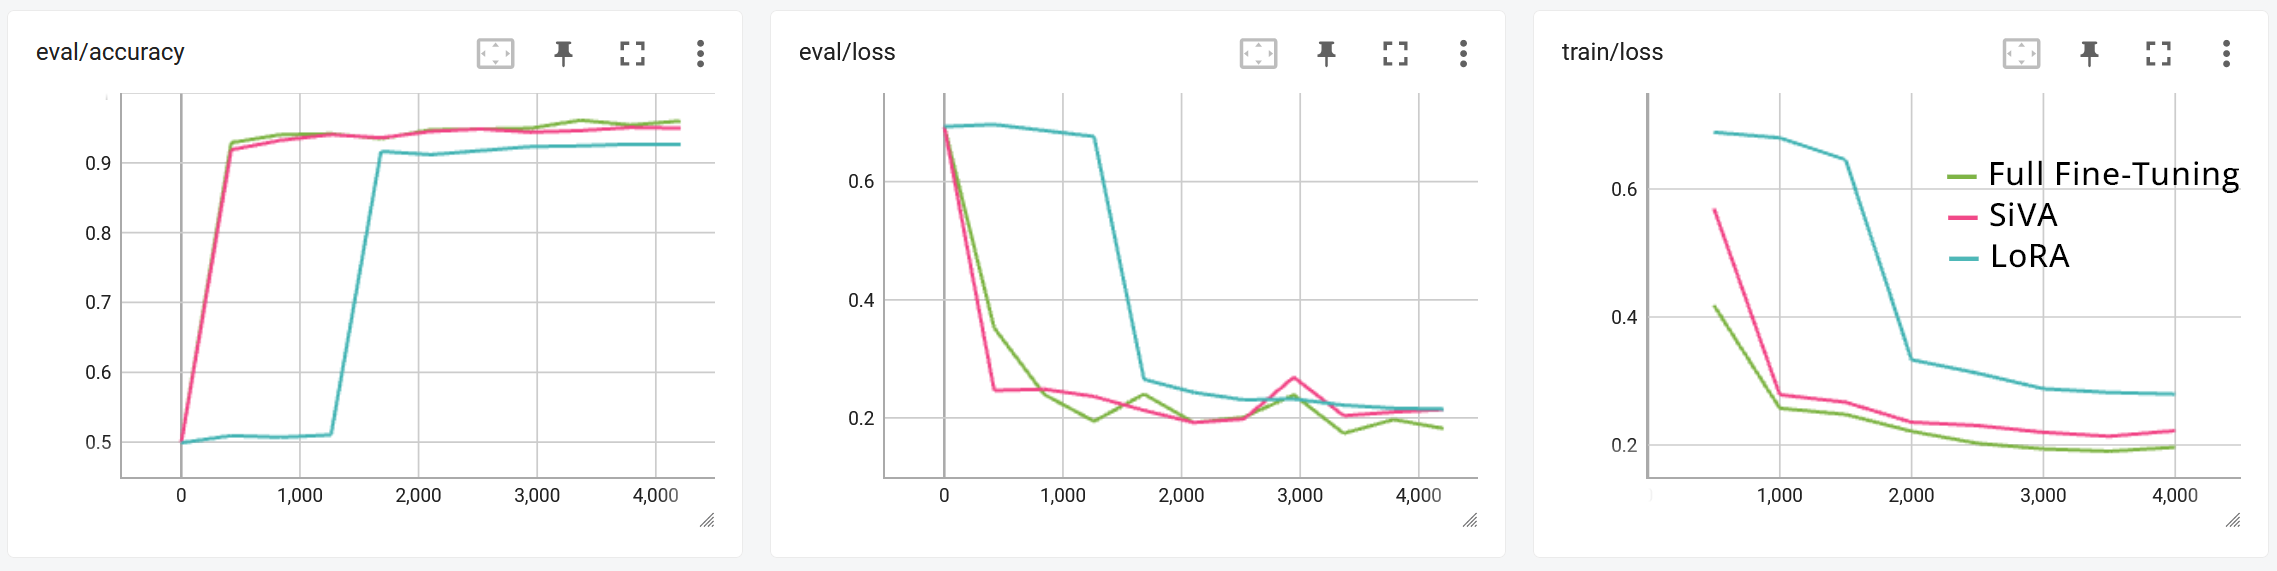
\includegraphics[width=\textwidth]{assets/images/siva-lora-training.png}
    \caption{The training graphs for full fine-tuning, SiVA, and LoRA for RoBERTa-large \cite{roberta} on the SST-2 \cite{wang2019glue} dataset for one epoch. Full fine-tuning and SiVA follow each other closely in all graphs while LoRA has worse performance. All the hyperparameters are the same, the original model initialization (including the head) is also the same. No smoothing applied.}
    \label{siva-lora-training}
\end{figure*}

\subsubsection{Forward Pass}
During the forward pass, training matrices are reconstructed and added to \(W_r\) to get the updated weight matrix without any loss of granularity from the lower-rank representation. For \(h = W_0 x\), the modified forward pass yields:

\begin{equation}
    h = W_r x + U_t \circ S_t V_t x
\end{equation}

\begin{figure}[htb]
    \centering
    \includesvg[width=\linewidth]{assets/images/lora-siva-forward-pass}
    \caption{Visual representation of the forward passes of LoRA and SiVA. In both figures, the trainable parts (\(A, B\) for LoRA and \(U_t, V_t\) for SiVA) are multiplied and added to the untrainable part to get the updated weight matrix. A linear transformation is applied with the resulting updated matrix to get the results. LoRA's trainable parts represent the change in the original matrix while SiVA's trainable parts represent the whole matrix.}
    \label{lora-siva}
\end{figure}

\Cref{lora-siva} shows the comparison between LoRA's and SiVA's forward passes. Recall that the modified forward pass of LoRA is formulized as \(h = W_0 x + B A x\). While \(A, B\) are same size matrices as \(U_t, V_t\); \(A, B\) represent only the change of the original matrix whereas \(U_t, V_t\) represent the whole matrix. 

\subsubsection{Optimal Hyperparameters}
SiVA introduces two new hyperparameters. For the training rank, we use \(r=4\) to reach the full fine-tuning performance on RoBERTa-large. We hypothesize that as the model size grows, \(r\) can get as low as \(1\) without losing any performance similar to LoRA. We use the number of output channels of \(W_0\) for the decomposition rank \(d\). Selecting a lower \(d\) reduces accuracy. Moreover, we experiment with training a subset of linear layers with SiVA and freezing the rest. We find the best balance between accuracy and efficiency when training only the key and query projection matrices in self attention.

\subsubsection{Comparing to LoRA and Full Fine-Tuning}
Similar to LoRA, training matrices of SiVA can be merged after training to get an unmodified model to remove any inference latency. They can also be swapped with other training matrices to modify the same base model for different fine-tuned tasks, eliminating the need for keeping multiple fine-tuned large models for different tasks. However, unlike LoRA, since SiVA does not have zero or random initialization, the optimization is easier and the training converges much faster.

As it can be seen from \Cref{siva-lora-training}, the training graphs of full fine-tuning and SiVA are almost identical, to the fluctuations of the unsmoothed graphs, whereas LoRA struggles to have any meaningful optimizations in the first quarter of the epoch due to the random and zero initializations of its layers. Even if we shift the LoRA graph left 1000 iterations to mitigate 50\% accuracy of the first quarter, we can observe that the accuracy and loss are still worse compared to full fine-tuning and SiVA. Due to the similarity of the training graphs of SiVA and full fine-tuning with the same hyperparameters, we claim that SiVA is analogous to full fine-tuning in a lower dimension.
